\documentclass[12pt,frontmatter,copyright,thesis]{usfmanus}
\usepackage[bottom=1in, left=1in, right=1in, top=1in]{geometry}

\usepackage{amsthm}
\usepackage{amsmath}
\usepackage{amssymb,alltt,url,verbatim}
\usepackage{float}
%\usepackage{caption}
\usepackage{graphics}
\usepackage{graphicx,leftidx}
\usepackage{epsfig}
\usepackage{fixltx2e}
\usepackage[english]{babel}
\usepackage{multirow}
\usepackage{enumitem}
\usepackage[]{algorithm2e}
\usepackage{scrextend}
\usepackage{pifont}
%\usepackage{mybeamer}
\setenumerate[0]{leftmargin=0.5in}
%\usepackage{float}
%\usepackage{tikz}
%\usepackage{color}




\newcommand{\eg}{\mbox{{\em e.g.}}}
\newcommand{\ie}{\mbox{{\em i.e.}}}
\newcommand{\viz}{\mbox{{\em viz.}}}

\title{Protocol Guided Analysis of Post silicon Traces Under Limited Observability}
\author{Yuting Cao}
\degree{Master of Science in Computer Science} 
\department{Computer Science and Engineering} 
\college{Engineering} 
\majorprofessor{Hao Zheng, Ph.D.} 
\majorproftitle{Associate  Professor, Department of Computer Science and Engineering} 
\members{MIMI, Ph.D. \and BIBI Ph.D.} 
\presentdate{To be determine}

\keywords{silicon, validation, trace, analysis, observability, signal selection}

\graddate{August, 2016} \copyrightyear{2016}

%\dedication{}

\acknowledgments{ 
I would like to thank my advisor Dr. Hao Zheng for his continuous support
and valuable suggestions for this research work. His insights on the topic was very 
valuable to me, especially his guidance and feedback has driven me in the proper direction 
of the research.

I would also like to thank my friend and family for supporting my academic career. 
}

\abstract{

We consider the problem of reconstructing system- level behavior of an SoC design from a partially observed signal trace. Solving this problem is a critical activity in post- silicon validation, and currently depends primarily on human creativity and insights. In this paper, we provide an algorithm to automatically infer system-level transactions from incomplete, ambiguous, and noisy trace data. We demonstrate the approach on a multicore virtual platform developed within the GEM5 environment.

}

\begin{document}

\chapter{Introduction}

In this thesis, we will present background information on the area of post-silicon validation and problems in the area in Chapter 2. Then in Chapter 3 an overview of current flow verification is presented. After that, we present our method in Chapter 4, 5 and 6 and implementation in Chapter 6. Chapter 7 will summarize our work and talk about our future works. All the flow specifications and protocols used in implementation process will be explained in Chapter 8.
\section{Silicon Validation}
Validation is the activity of ensuring a product satisfies its specifications, compatible with related software and hardware and meets user expectations. ~\cite{validationWall}

Silicon Validation is needed because numbers of processor bug are growing and bugs are becoming more diverse and complex.

 \section{Pre- and Post-silicon Validation}


The product development cycle often tends to be linear. The phase will start with planning and architecture, followed by RTL and schematic creation and architectural and functional validation (pre-silicon validation) leading up the tape out. Post-silicon validation will start when the first chip arrives. And eventually when all specification are meet, the product will be released to be market. ~\cite{validationWall}

Pre-silicon validation aims to verify the architecture design before 
it's implemented on an actual chip. It's mainly done at RTL level on simulators, FPGAs, or emulators. 
During pre-silicon validation, the cause of fixing bug is relatively low. 
Any bugs can be fixed by RTL modification and small amount of time
The downside is, pre-silicon validation is limited by its speed and coverage. 
Simulators are usually very slow and only suitable for small portions
of the design. FPGAs are up to 3 orders of magnitude faster. Emulator can combine multiple FPGAs
to work on a larger portion of the RTL design with cause of limited speed. All the limitations makes
pre-silicon only able to verify part of the system. 


Post-silicon validation makes use of pre-production silicon
integrated circuit (IC) to ensure that the fabricated system
works as desired under actual operating conditions with real
software.  Since the silicon executes at target clock speed,
post-silicon executions are billions of times faster than
RTL simulations, and even provide speed-up of several orders
of magnitude over other pre-silicon platforms (\eg, FPGA,
system-level emulation, etc.).  This makes it possible to
explore deep design states which cannot be exercised in
pre-silicon, and identify errors missed during pre-silicon
validation and debug.  However, limited pin-out and
other architecture factors makes it impossible to have full observability of the system.
Only a limited number of signals can be observed and traced. This limitation 
brings challenge in both detecting bugs and debugging process. 


\section{Related Work}

Paper ~\cite{validationWall} goes through the definition of
silicon validation and reason why it is important. Together with 
current techniques used for pre- and post-silicon validation.

Our work is closely related to communication-centric and
transaction based debug.  An early pioneering work is
described in~\cite{Goossens2007NOCS}, which advocates the
focus on observing activities on the interconnect network
among IP blocks, and mapping these activities to
transactions for better correlation between computations and
communications.  Therefore, the communication transactions,
as a result of software execution, provide an interface
between computation and communication, and facilitate
system-level debug.  This work is extended
in~\cite{Vermeulen2009VLSI-DAT,Goossens2009DATE}.  However,
this line of work is focused on the network-on-chip (NoC)
architecture for interconnect using the run/stop debug
control method.

A similar transaction-based debug approach is presented
in~\cite{Gharehbaghi2012ISQED}.  Furthermore, it proposes an
automated extraction of state machines at transaction level
from high level design models.  From an observed failure
trace, it performs backtracking on this transaction level
state machine to derive a set of transaction traces that
lead to the observed failure state.  In the subsequent step,
bounded model checking with the constraints on the internal
variables is used to refine the set of transaction traces to
remove the infeasible traces.  This approach requires user
inputs to identify impossible transaction sequences, and may
not find the states causing the failure if the transaction
traces leading to the observed failure state is long.
Backtracking from the observed failure state requires
pre-image computation, which can be computationally
expensive.  A transaction-based online debug approach is
proposed in~\cite{Dehbash2014} to address these issues.
This approach utilizes a transaction debug pattern
specification language~\cite{Gharehbaghi2009ICCD} to define
properties that transactions should meet.  These transaction
properties are checked at runtime by programming debug units
in the on-chip debug infrastructure, and the system can be
stopped shortly after a violation is detected for any one of
those properties.  In this sense, it can be viewed as the
hardware assertion approaches in~\cite{Boule2007ISQED}
elevated to the transaction level.

In~\cite{Singerman2011DAC}, a coherent workflow is described
where the result from the pre-silicon validation stage can
be carried over to the post-silicon stage to improve
efficiency and productivity of post-silicon debug.  This
workflow is centered on a repository of system events and
simple transactions defined by architects and IP designers.
It spans across a wide spectrum of the post-silicon
validation including DFx instrumentation, test generation,
coverage, and debug.  The DFx instruments are automatically
inserted into the design RTL code driven by the defined
transactions.  This instrumentation is optimized for making
a large set of events and transactions observable.  Test
generation is also optimized to generate only the necessary
but sufficient tests to allow all defined transactions to be
exercised.  Moreover, coverage for post-silicon validation
is now defined at the abstract level of events and
transactions rather than the raw signals, and thus can be
evaluated more efficiently.  In~\cite{Abarbanel2014DAC}, a
model at an even higher-level of abstraction, {\em flows},
is proposed.  Flows are used to specify more sophisticated
cross-IP transactions such as power management, security,
etc, and to facilitate reuse of the efforts of the
architectural analysis to check HW/SW implementations.




\section{Motivation}

Post-silicon validation is a critical
component of the design validation life-cycle for modern
microprocessors and SoC designs.  Unfortunately, it is also
a highly complex component, performed under aggressive
schedules and accounting for more than $50\%$ of the overall
design validation cost~\cite{Patra2007}.  Consequently, it
is crucial to develop techniques for streamlining and
automating post-silicon validation activities.



%%explainging why trasfering to system level  transaction
A key component of post-silicon validation of SoC designs is
to correlate traces from silicon execution with the intended
system-level transactions.  An SoC design is typically
composed of a large number of pre-designed hardware or
software blocks (often referred to as ``intellectual
properties'' or ``IPs'') that coordinate through complex
protocols to implement the system-level behavior.  Any
execution trace of the system involves a large number of
interleaved instances of these protocols.  For example,
consider a smartphone executing a usage scenario where the
end-user browses the Web while listening to music and
sending and receiving occasional text messages.  Typical
post-silicon validation use-cases involve exercising such
scenarios. 

 An execution trace would involve activities from
the CPU, audio controller, display controller, wireless
radio antenna, etc., reflecting the interleaved execution of
several communication protocols.  On the other hand, due to
observability limitations, only a small number of
participating signals can be actually traced during silicon
execution.  Furthermore, due to electrical perturbations,
silicon data can be noisy, lossy, and ambiguous.
Consequently, it is non-trivial to identify all
participating protocols and pinpoint the interleaving that
results in an observed trace.

%%explainging why should be communication centric verification
With the increasing complexity of modern SoC designs nowadays, 
debugging protocols inside IP
blocks by themselves is not enough anymore. The complexity
of the SOC increasingly resides in the interactions between
the IP blocks. 
Therefore, debug must be conducted
at a higher system level, where the computation threads
and communication threads interact.
 Because the interconnect
implements the communication, and hence the synchronization
between the IP blocks is the natural focus for system-level
debug~\cite{Goossens2007NOCS}.

In this thesis, we consider the problem of reconstructing
protocol-level behavior from silicon traces in SoC designs.
Given a collection of system-level communication protocols
and a trace of (partially observed) hardware signals, our
approach infers, with a certain measure of confidence, the
protocol instances (and their interleavings) being exercised
by the trace.  The approach is based on a formalization of
system-level transactions via labeled Petri-Nets, which are
capable of describing sequencing, concurrency, and choices
over system events.  We develop algorithms to infer
system-level transactions from traces with missing, noisy,
and ambiguous signal values.  We demonstrate our approach on
a multicore virtual platform constructed within the GEM5
environment~\cite{Binkert2011} and another RTL model written in VHDL.



\chapter{Background}
 \section{Representations of SoC Protocols }
  
 In software engineering field, there are two approaches for representing the system protocols: informal
 and formal representation.
  Informal representation usually use common 
  graphical notation for representation for better understandability and easier communication with the client. 
The formal representation is usually built on strong mathematical notations and proofs for
more automated verification purpose.

System development usually need to create protocol in both formal and informal formats. 
Informal format is mostly used for communications and formal format for verification purpose. 
Usually it requires manual translation of an informal description to a formal description, which 
requires massive amount of time and effort when system growing larger and more complicate. 
 ~\cite{lsctocpn} introduced a tool translating informal formal Live Sequence Chart
 into formal format of Colored Petri-net, which can be great help for future research.


 An SoC design involves integration of a number of IPs that
communicate through complex protocols.  Such system-level
protocols are typically specified in architecture documents
as message flow diagrams.  For this thesis, we use the words
``protocol'' and ``flow'' interchangeably.

\begin{figure}[h]
\centering
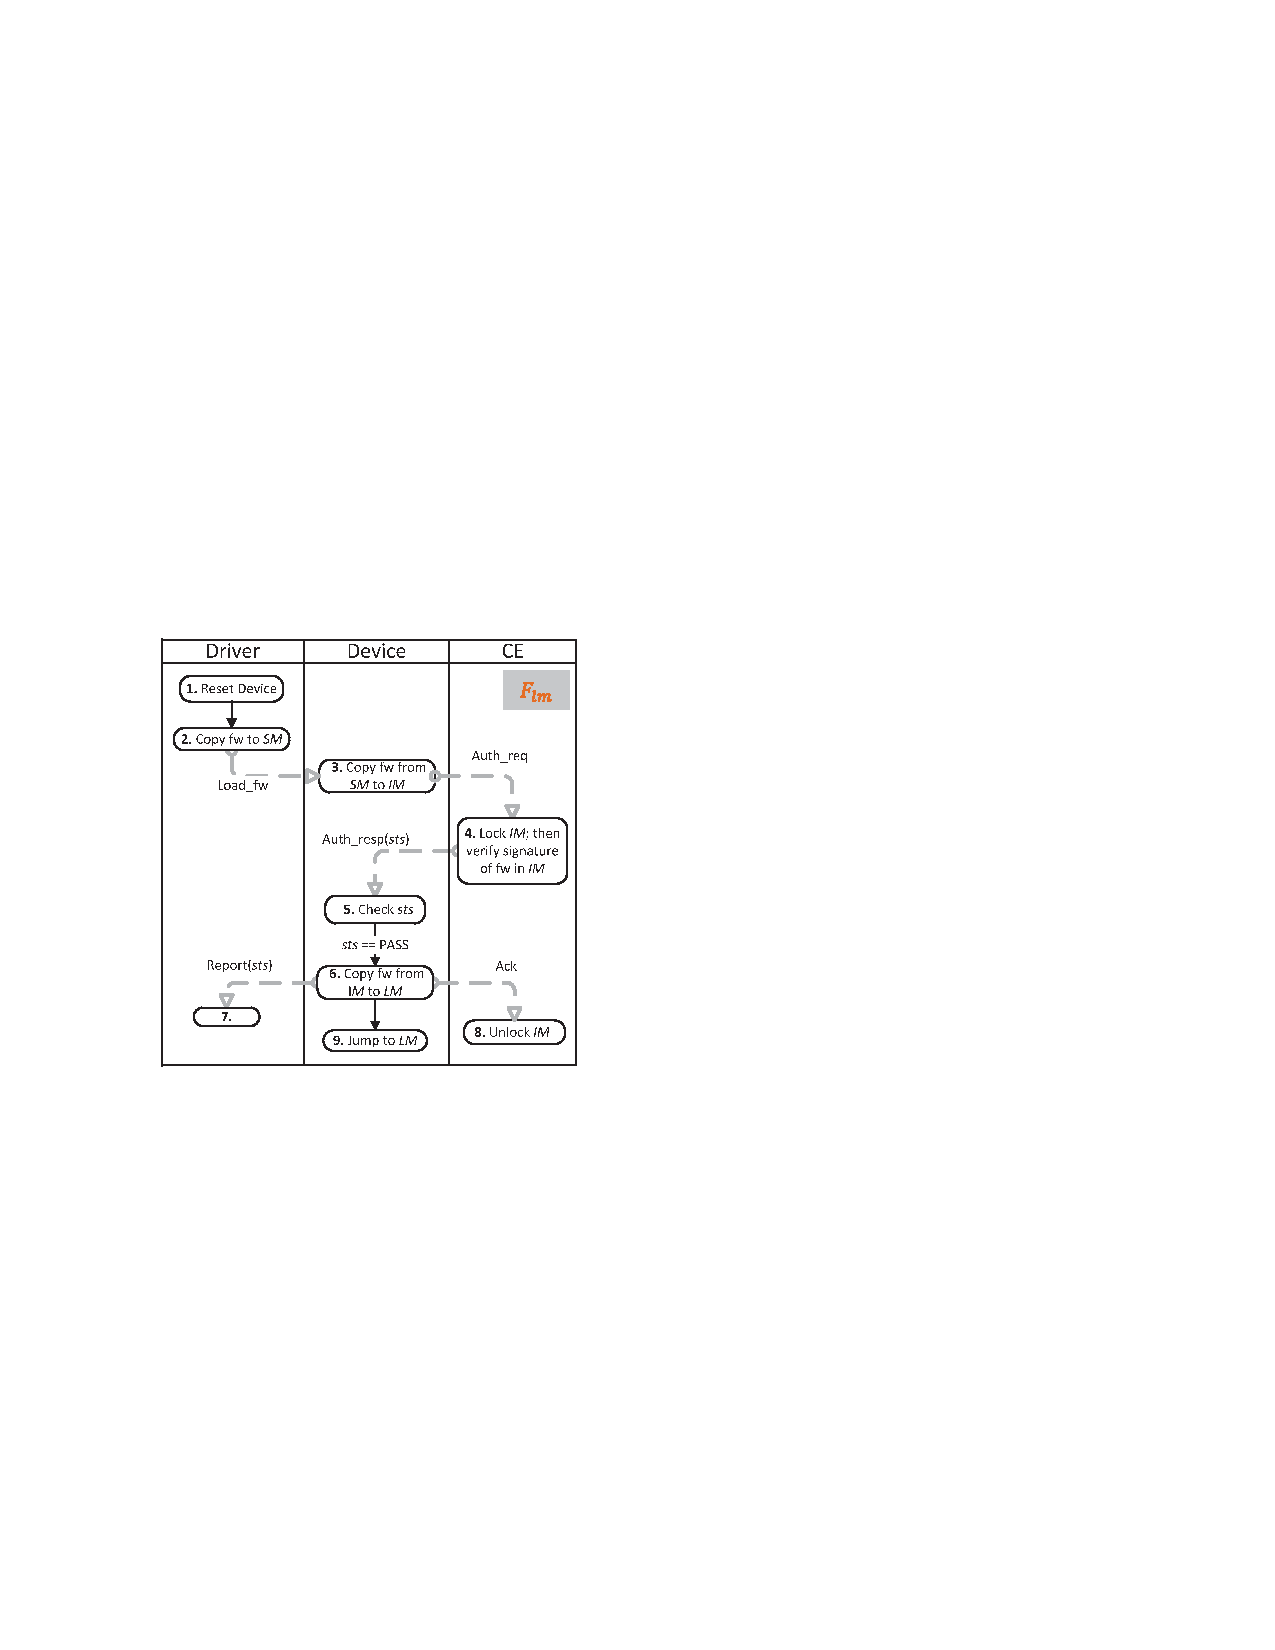
\includegraphics[width=0.5\textwidth]{figures/bpmn-flow-ex}
\label{flowa}
\caption{A graphical representation of a SoC firmware load protocol~\cite{Krstic14HOST}.}
\end{figure}

Fig~\ref{flowa} shows one diagram for a protocol
to authenticate and load a firmware during system boot for
firmware upgrade.  To start this protocol, the Driver will reset Device and copy the needed
firmware to a place in System Memory (SM) and notice the Device to load it. With the location of firmware
provided from Driver, Device can retrieve firmware to Isolated Memory (IM) and sends the message $Auth\_req $
to Crypto-engine (CE), providing the location of the copied firmware, and asking for authentication. After verifying 
signature of firmware in IM, CE will reply with 
PASS/FAIL status ($sts$). 
Upon receiving the PASS $sts$, Device sends report message to Driver and acknowledge message
to CE and then jump to the firmware from Local Memory (LM)

Currently our research is only for verification purpose and our system is too simple
to need two formats of specification, so we only use the formal format of Labeled Petri-net, which is introduced 
in section \ref{petri}. Section \ref{diagram} will give a brief explanation of sequence diagram as an 
example of informal representation.


\section{Sequence Diagram} \label{diagram}
Sequence Diagram represents the
 life cycle of an processor and the interactions between them.
%% Life cycle of an object is represented by a vertical line
 %% and the interaction between objects is represented by 
 %% a horizontal line with an arrow pointing towards the receiver object.
Common used sequence diagram include UML sequence diagram, message sequence 
diagram and live sequence diagram.~\cite{lsctocpn}
 
\begin{figure} [h]
\centerline{
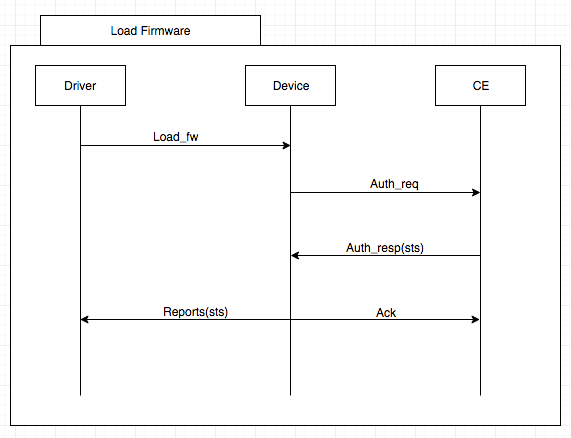
\includegraphics[width=5in]{livesc.png}}
\caption{Protocol in Fig.~\ref{flowa} represented in graphical LSC }
\label{livesequence}
\end{figure}
 Fig.~\ref{livesequence} shows the live sequence chart representation of protocol from Fig.~\ref{flowa}.
 In this graph we can clearly see the sequence of the communication between each IP.

%%At this time, the initiator sets the $data$ line and then asserts 
%%the $valid$ signal. Once the target samples the $valid$ signal asserted, 
%it is free to sample the value on the $data$ line. 
%After zero or more clock ticks, the target then asserts $ack$ to acknowledge 
%receipt of the data value. At this point, a single clock tick must occur before
 %the $initiator$ can deassert $valid$ and the $target$ can deassert $ack$ since the 
 %data transfer officially occurs on the clock edge on which both $valid$ and $ack$ 
 %are asserted. 
% Again, zero or more clock ticks may occur before the transaction
  %exits by leaving the interface in a state in which $valid$ and $ack$ are both 
  %deasserted. ~\cite{Bunker2005}
  
  
  
\section{Labeled Petri-Nets} \label{petri}
Labeled Petri-nets (LPN) is a formalization of state transition 
systems that is capable of describing sequencing, concurrency, and choices.  
Compared with informal representation, it can be verified using mathematical techniques
and tools.
 %--- LPN definition with levels
 
 Formally, an LPN is a tuple $(P, T, s_0, E, L)$  where
 \begin{itemize}
 \item $P$ is a finite set of places,
 \item $T$ is a finite set of transitions,
 \item $s_0$ is the set of initially marked places, also referred to as the initial marking.
 \item $E$ is a finite set of events,
 \item $L$ is a labeling function that maps each transition $t \in T$ to an event $e \in E$. 
 \end{itemize}
 
 For each transition $t \in T$, its preset, denoted as $\bullet{t} \subseteq P$, is the set of places connected to $t$, and its postset, denoted as $t\bullet \subseteq P$, is the set of places that $t$ is connected to.  A marking of a LPN is a set of places marked with tokens, and it is alsoreferred to as a state of a LPN. The initia marking $init$ is 
 also the initial state of the LPN.

 The operational semantics of a LPN is defined by transition executions.  
 A transition can be executed after it is {\em enabled}.  
 A transition $t \in T$ is enabled in a state $s$ if every place in its preset is included in the marking, i.e. $\bullet{t} \subseteq s$.  Execution of $t$ results in a new state $s'$ such that 
 \[
 s' = (s - \bullet{t}) \cup t\bullet,
 \]
 and the emission of event $e$ labeled for $t$. 

\begin{figure}
\label{changedb}
\centering
    \includegraphics[width=0.7\textwidth]{try}
  \caption{LPN formalization.
  Each event has a form of $\langle {\tt src, dest, cmd}
  \rangle$ where ${\tt cmd}$ is a command sent from a source
  component ${\tt src}$ to a destination component ${\tt
    dest}$. The solid black places without outgoing edges
  are {\em terminals}, which indicate termination of
  protocols represented by the LPNs.}
\end{figure}


 The communication protocol in the BMPN shown
 in~Fig.~\ref{flowa} is represented by the LPN
 shown in~Figure~\ref{changedb}.  In this and the
 following figures for LPNs, the labeled circles denote
 places, and the labeled boxes denote transitions.  Each
 transition is labeled with its name and the associated
 event.  Each event has a form of $\langle {\tt src, dest,
   cmd} \rangle$ where ${\tt cmd}$ is a command sent from a
 source component ${\tt src}$ to a destination component
 ${\tt dest}$. 
 (Another form of event used in our RTL model implementation
 is $\langle {\tt src, dest, cmd, addr} \rangle$ where $addr$ is an unique id for
 each flow instance, this can be used to make flow interpretation easier.)
  The solid black places without outgoing edges
 are {\em terminals}, which indicate termination of protocols
 represented by the LPNs.  The initial marking is
 $\mathit{s_0} = \{p_1\}$.  In this LPN model, only the
 communication portion of the BPMN specification is
 represented while the computation portion is ignored.


  %%@COMMENT This example is for LPNs with guards.
 %The above protocol specification can be made more precise by describing how component~2 would respond without using non-determinism.  For example, the system architect may wish to specify that component~2  responds with $\mathit{msg_2}$ to every sequence of two $\mathit{msg_1}$ for five such sequences in a row.  On the sixth such sequence, component~2 responds with $\mathit{msg_3}$.  The LPN modeling such protocol is shown in Figure~\ref{fig-flow-ex-2}.  An alternative without using auxiliary variables in the transition predicates is by unrolling the loops for the specified number of times; however this would result in a larger and more complex LPN.  


 

\chapter{Flow Guided Trace Interpretation}

 In this chapter,
 we describe a trace analysis method where the observed
 signal traces are interpreted at the level of system
 flows. In general, the trace analysis can offer
 debuggers a structured view of communications among the
 IP blocks during the SUD execution by deriving the types
 and numbers of system flows activated during SUD
 executions from the observed signal traces.

We formalize the trace interpretation problem in terms of labeled Petri-nets,
 and discuss algorithms to address the problem.
  For pedagogical reasons, here we assume full
   observability of all hardware signals involved in the flow events. 
  In the next chapter we will extend the approach
   to consider partial observability.

\section{Post-silicon Trace Analysis}
 In a typical validation setting, the system under debug
 (SUD) is executed in a test environment until it is
 terminated by the test environment or the system crashes
 due to a failure.  During the execution, a trace on a
 small number of observable signals is streamed off the
 chip for debugging.  
The off-chip analysis
includes two broad phases:
\begin{itemize} 
\item trace abstraction that translate signal traces into flow traces
\item trace interpretation that translate flow traces into flow execution scenarios
\end{itemize}
Trace abstraction maps the
hardware trace into higher-level architectural constructs,
\eg, messages, operations, etc. A message such as {\tt
  Authorization request} may be implemented in hardware
through a Boolean or temporal combination of specific
hardware signals in the NoC fabric between {\tt Device} and
{\tt CE}, \eg, as a sequence containing a header, a specific
value of a sequence of data words, etc.  We will refer to
such architectural constructs as {\em protocol events} or
{\em flow events}.  Note that due to limited observability,
it may not be possible to map a given set of (observed)
hardware signals uniquely to a flow event.  Finally, the
trace may be a result from several instances of the same
protocol executing concurrently, \eg, a firmware
authentication protocol may be invoked when another instance
of the protocol has not completed.



Trace interpretation entails mapping a sequence of flow events created
during trace abstraction to system-level protocols in order
to identify the set of protocol instances (and
interleavings) responsible for creating the observed
behavior. The trace interpretation takes a finite trace of flow events
 resulting from the trace abstraction and a set of system
 flows in LPNs $\vec{F}$, and generates a set of possible
 system flow execution scenarios, which is defined in next section.
   A flow execution scenario
 indicates that at a certain point of SUD execution, what
 types of flows and the number of instances of a particular
 flow are activated and their corresponding current states.

The trace may identify a problem in the protocols
themselves, \eg~an interleaving of some protocol executions
may lead to an unexpected message being sent or cause the
system to crash.  More commonly, one finds a bug in the {\em
  implementation} of the protocol, \ie, a trace inconsistent
with any possible interleaving of the protocol executions.
Identifying these problems involves significant human
expertise, and can often take days to weeks of effort.



\section{Flow Execution Scenarios}
 The set
of system flows is a collection ${\vec{F}}$ of
LPNs.  A {\em flow execution scenario} is defined as a
set $\{(F_{i,j}, s_{i,j})\}$ where $F_{i,j}$ is the
$j$th instance of flow $F_i \in {\vec{F}}$, and $s_{i,j}$ is
a state of $F_{i,j}$.  A flow execution scenario indicates
the set of protocols and the number of instances of a
particular protocol are activated and their corresponding
current states.  Since we assume full observability, we view
an {\em observed trace} $\rho = e_1e_2\ldots e_n$ as a
sequence of flow events.  
 Let
$\mathit{accept(F_{i,j}, s_{i,j}, e)}$ be a function that
determines if event $e$ can be emitted by $F_{i,j}$ in state
$s_{i,j}$.  Formally, $\mathit{accept(F_{i,j}, s_{i,j}, e)}$
returns $(F_{i,j}, s'_{i,j})$ where $s'_{i,j} = (s_{i,j} - \bullet t)
\cup t\bullet$ if there exists a transition
$t$ in $F_i$ such that $L(t) = e$ and $\bullet t \subseteq
s_{i,j}$.  It returns $(F_{i,j}, \emptyset)$ otherwise.

Given an observed trace $\rho$, the
goal of trace interpretation is to construct a set of
candidate flow execution scenarios whose execution can
create the sequence of events in $\rho$.  
Such that $\rho$ is the result of executing 
the flow instances in those execution scenarios by following 
the corresponding LPN operational semantics. We call such execution scenarios $compliant$ 
with $\rho$.


\section{Flow Guided Trace Interpretation Algorithm}
Given an observed flow trace $\rho$ and the set $\vec{F}$ of flows,
Algorithm~\ref{algo:compliance} provides a basic procedure for
computing a set of compliant flow execution scenarios. 
The algorithm operates by keeping track (in variable
$\mathit{Scen}$) of a set of candidate flow execution scenarios
compliant with each prefix of $\rho$.  At each iteration,
for each event $e_h$ in the observed trace, we
update $Scen$ by either extending a member of
$\mathit{scen}$ or initiating a new flow instance for 
each $scen \in Scen$ with respect to $e_h$ in every possible way.
If $e_h$ cannot be accepted by any existing or new flow instances, 
then we report that the trace is {\tt  inconsistent} with $\mathit{Scen}$, \ie, 
the execution scenario $\mathit{Scen}$ is not compliant with
$\rho$.

\begin{algorithm}[h]
\setstretch{0.9}
\DontPrintSemicolon
Create an empty scenario $scen$\;
$\mathit{Scen} = \{scen\}$\;
\ForEach {$h, \; 1 \leq h \leq n $} {
	$\mathit{found} \gets {\tt true}$ \;
	$Scen' = \emptyset$\;
	\ForEach {$scen \in Scen$} {
  		\ForEach {$(F_{i,j}, s_{i,j}) \in \mathit{scen}$} {
    		\If {$((F_{i,j}, s'_{i,j}) \gets (\mathit{accept}(F_{i,j}, s_{i,j}, e_h) )) \cap (s'_{i,j}\neq \emptyset )$} {
				Let $scen'$ be a copy of $scen$\;
      		$\mathit{scen'} \gets \mathit{scen'} - (F_{i,j}, s_{i,j})) \cup (F_{i,j}, s'_{i,j}$\;
      		$\mathit{Scen'} \gets \mathit{scen'} \cup \mathit{Scen'}$\;
      		$\mathit{found} \gets {\tt false}$ \;
    		}
  		}
  		\ForEach {$F_i \in \vec{F}$} {
      	create a new instance $F_{i, j+1}$ \;
      	\If {$((F_{i,j+1}, s'_{i,j+1})\gets\mathit{accept}(F_{i,j+1},\mathit{init}_{i,j+1}, e_h)) \cap(s'_{i,j+1}\neq \emptyset ) $} {
    			Let $scen'$ be a copy of $scen$\;
				$\mathit{scen'} \gets \mathit{scen'} \cup (F_{i,j+1}, s'_{i,j+1})$ \;
				$\mathit{Scen'} \gets \mathit{scen'} \cup \mathit{Scen'}$\;
        		$\mathit{found} \gets {\tt false}$ \;
      	}
    	}
	}
  \If {$\mathit{found} == {\tt true}$} {
    \Return ${\tt Inconsistent}$\;
  }
  $Scen = Scen'$\;
}
\Return $\mathit{Scen}$ \;
\caption{$\textsc{Check-Compliance}(\vec{F}, \, \rho)$}
\label{algo:compliance}
\end{algorithm}


 Given a trace of flow events $\rho = e_1e_2\ldots e_n$, the
 trace interpretation algorithm starts with an empty set of
 of flow execution scenario $\mathit{Scen} = \emptyset$.
 Then, for each $e_h$ where $1 \leq h \leq n$ starting $h=1$,
 and for each $\mathit{scen} \in \mathit{Scen}$, the
 following two steps are performed.
 \begin{description}
 \item[Step 1]~~For each $(F_{i,j}, s_{i,j}) \in
   \mathit{scen}$, if $\mathit{accept}(F_{i,j}, s_{i,j}, e_h)
   = (F_{i,j}, s'_{i,j})$, create a new scenario
   $\mathit{scen}' = (\mathit{scen} - (F_{i,j}, s_{i,j}))
   \cup (F_{i,j}, s'_{i,j})$, which is added into
   $\mathit{Scen}'$.

 \item[Step 2]~~For each $F_i \in \vec{F}$, create a new
   instance $F_{i, j+1}$.  If $\mathit{accept}(F_{i,j+1},
   \mathit{init}_{i,j+1}, e_h) = (F_{i,j+1}, s'_{i,j+1})$,
   create a new scenario $\mathit{scen}' = \mathit{scen} \cup
   (F_{i,j+1}, s'_{i,j+1})$, which is added into
   $\mathit{Scen}'$.
 \end{description}
After $e_h$ is processed, $Scen = Scen'$, and the above two
 steps repeat for the next event $e_{h+1}$.

 If every events in $\rho$ is successfully mapped to some
 flow instance, this algorithm returns a set of flow
 execution scenarios such that every flow execution scenario on is compliant to $\rho$.
   On the other hand, inconsistent events can
 also be encountered.  An event $e$ is \emph{inconsistent} if
 for each flow execution scenario $\mathit{scen} \in
 \mathit{Scen}$, the following two conditions hold.

 \begin{enumerate}
 \item For each $(F_{i,j}, s_{i,j}) \in \mathit{scen}$,
   $\mathit{accept}(F_{i,j}, s_{i,j}, e_h) = \emptyset$,
 \item For each $F_i \in \vec{F}$, $\mathit{accept}(F_{i},
   \mathit{init}_{i}, e_h) = \emptyset$.
 \end{enumerate}

 An inconsistent event is the one produced by SUD execution
 but cannot be mapped to any flow instances no matter how the
 trace prior to event $e$ is interpreted.  Inconsistent
 events indicates possible causes of system failures.

 Based on the above discussion, the trace interpretation
 algorithm generates two pieces of information: 1) a set $G$ of
 flow execution scenarios each of which is compliant with the observed trace, 2) a pair $B$,
 which includes a flow execution scenario and
 an corresponding inconsistent event.  The pair $B$ provide valuable
 information for debuggers to root cause system failures.
 The algorithm returns either G or B.  With the full
 observability, the set $G$ includes a single flow execution
 scenario derived for a trace.  In reality, it is always the
 case that the SUD is only partially observable.  Therefore,
 due to the lack of information for precise interpretation, a
 set of flow execution scenarios is typically derived for a
 given trace as the result of the trace analysis.

\section{Illustration}
To illustrate the basic idea of the trace analysis method, consider the system flow shown in 
Fig.~\ref{changedb}. Let $F_1$ denote such flow.
Suppose that the following flow trace is abstracted from an
observed signal trace.
\[
	t_1\;t_2\;t_1\;t_2\;t_3\;t_3\;t_4\;t_5\;t_5\;t_4\ldots
\]  
This trace is interpreted from the first event to the last in order to derive all possible flow execution
 scenarios.
Here transition names in the LPN are used to represent the 
flow events in the trace.  
At the begininng, the first event $t_1$ is process. 
According to the flow specification $F_1$, 
we know that one instance of such flow $F_1$, $F_{1,1}$, is activated by the SUD 
as $\mathit{accept}(F_{1,1}, init_1, t_1) = (F_{1,1}, \{p_2\})$ where $\mathit{init} = \{p_1\}$ is the initial state of $F_1$.  As the result, the flow execution scenario after interpreting the first event $\mathit{msg_1}$ is $\{(F_{1,1}, \{p_2\})\}$.  

Next, the second $t_1$ is interpreted. This event is the continuing execution of 
$F_{1,1}$ as $\mathit{accept}(F_{1,1}, {p_2}, t_2) = (F_{1,1}, \{p_3\})$.
Next event $t_1$ will activate another instance of flow $F_1$, $F_{1,2}$. And event $t_2$
 after that is the continuing event of $F_{1,2}$, resulting in
the following flow execution scenario
\[
	\{(F_{1,1}, \{p_3\}),~(F_{1,2}, \{p_3\})\}.
\]
For the fifth event $t_3$, it can be the result of continuing execution of $F_{1,1}$ 
or $F_{1,2}$. Therefore,
two execution scenarios can be derived as showed below.
\[
\begin{array}{l}
	\{(F_{1,1}, \{p_4\}),~(F_{1,2}, \{p_3\})\} \\
	\{(F_{1,1}, \{p_3\}),~(F_{1,2}, \{p_4\})\}.
\end{array}
\]
After handing the next event $t_3$, the above two execution scenarios
are reduced to the one as shown below.
\[
	\{(F_{1,1}, \{p_4\}),~(F_{1,2}, \{p_4\})\}.
\]
Using Algorithm~\ref{algo:compliance} to handle the
remaining four events, the following execution scenario is
derived.
\[
	\{(F_{1,1}, \{p_5, p_6\}),~(F_{1,2}, \{p_5, p_6\})\}
\]




\chapter{Trace Analysis Under Partial Observability}

In hardware that implements a given system flow
 specification, a flow event is assumed to be implemented as an event or a
 sequence of events on a set of signals.  
 However, in post-silicon verification, it is impossible to have full observability of all 
 signals. There are two reasons that result in such limitation:
 \begin{itemize}
 \item Limitation of the interface: there are limited number of pins on the boundary of chip available for observation.
 \item Speed frequency difference: the big speed frequency gap between chip and interface may lead to data lost. 
 \end{itemize}
  In this chapter, we discuss how the
 trace analysis method presented in the previous chapter can be adapted to deal
 with signal traces of partial observability. A signal event is defined as a state on or an
assignment to a set of signals.
Hereafter, the term {\em flow traces} is used to refer to
traces of flow events. 
 
In general, a signal trace of partial observability is a set of signal events
with some signal value unknown. In this case, we will consider all possibilities for that signal value, 
each corresponding to a fully observable signal trace. Thus we can say that one partial observable signal
 trace can be mapped to a set of fully observable signal traces.
We take the following signal trace with signal $c$'s value missing as an example.
\[
\begin{array}{cl}
 ab\textvisiblespace\\
\end{array}
\] 
There are two possible values for signal $c$: $c$ or $\bar{c}$. To consider
both of the possibilities, we will have two fully observable signal traces: 
\[
\begin{array}{cl}
 abc\\
 ab\bar{c}\\
\end{array}
\] 

In the following, we discuss two cases for trace abstraction on
partial observability: mapping a single signal event to a
flow event or mapping a sequence of signal events to a flow
event.   

\section{Mapping Individual Signal Event to Flow Event}
Consider the following example for
the first case.  Suppose that there are three flow events:
$e_1$, $e_2$, and $e_3$, which are implemented in hardware
by the signal events shown in the list below.  We use
Boolean expressions to represent signal events for the
discussion.
\[
\begin{array}{cl}
e_1: & abc\\
e_2: & \bar{a}bc\\
e_3: & a\bar{b}c
\end{array}
\] 
Suppose that only signals $b$ and $c$ are observable, and we
obtain the following trace:
\[
bc\ bc \ \bar{b}c
\]
With all possibilities of signal $a$ considered, we will have the following 
fully observable signal traces:
obtain the following trace:
\[
\begin{array}{cl}
trace_1: & abc\ abc \ a\bar{b}c\\
trace_2: & abc\ abc \ \bar{a}\bar{b}c\\
trace_3: & abc\ \bar{a}bc \ a\bar{b}c\\
trace_4: & abc\ \bar{a}bc \ \bar{a}\bar{b}c\\
trace_5: & \bar{a}bc\ abc \ a\bar{b}c\\
trace_6: & \bar{a}bc\ abc \ \bar{a}\bar{b}c\\
trace_7: & \bar{a}bc\ \bar{a}bc \ a\bar{b}c\\
trace_8: & \bar{a}bc\ \bar{a}bc \ \bar{a}\bar{b}c\\
\end{array}
\]
During trace abstraction, only in $trace_1$ and $trace_2$,
the first two signal events $abc$
can be mapped to $\{e_1, e_2\}$.
After that, the third signal event in $trace_2$ can not be mapped to any
flow event, therefore only $trace_1$ is considered here, mapping $a\bar{b}c$ to
flow event $\{e_3\}$.
Therefore,
this signal trace is abstracted to four flow traces, $\{e_1,
e_2\} \times \{e_1, e_2\} \times \{e_3\}$.
Hereafter, we will not repeat the process of mapping partial observed signal trace to set of 
fully observed signal traces. 


\section{Sequence of Signal Events}
Next, we consider the case where a flow event is mapped from
a sequence of signal events.  Now suppose that two other
flow events are implemented by sequences of signal events as
defined in the list below.
\[
\begin{array}{cl}
e_4: & abc\ \bar{a}bc\\
e_5: & abc\ abc\ abc\ \bar{a}bc\\
\end{array}
\] 
Given an observed trace of the same observability shown below
\[
bc\ bc\ bc \ bc,
\]
Flow $e_4$ can be mapped to the first two $bc$s, the two $bc$s in the middle or in the end, or the whole trace can be mapped
to just one $e_5$ flow instance. It is abstracted to the following flow traces.
\[
e_4e_4,\; \textvisiblespace e_4 \textvisiblespace,\;  e_4 \textvisiblespace \textvisiblespace,\;  \textvisiblespace \textvisiblespace e_4, \; e_5
\] 

where $\textvisiblespace$ denotes signal events that are not
mapped to any flow events.  Note that the above abstraction
leads to three distinct flow traces as the middle three
correspond to the same flow trace.


\section{Sequence of Gapped Signal Events}
Most of the time, the speed of data generation is much faster
than speed of pins outputting data. Therefore, when there are big amount of 
data generated, there is a possibility of data loss, leaving a gap between the signal traces.

Here we will use flow event $e_4$ and $e_5$ from previous section as an example. We assume 
the same observability.
Given an observed trace of the same observability shown below
\[
\begin{array}{cl}
bc\ \textvisiblespace\  \textvisiblespace\ bc\ bc\
\end{array}
\]
The $\textvisiblespace$s in the signal traces indicate the gap with maximum two signal events. 
For this situation we will go through each $\textvisiblespace$, considering all possibility for that signal
event and try to map it to flow event. The process will stop when the newly mapped flow event can be 
mapped to an existing scenario or start a new scenario. If the mapped flow event is in consistent even
after considering the last $\textvisiblespace$, then we conclude there is an error.

For this example, we consider the first $\textvisiblespace$. There are four possibilities: $bc\ b\bar{c}\ \bar{b}c\ \bar{b}\bar{c}$.
Only $bc$ can be accepted since flow event $e_4\ and\ e_5$ only accept $bc$.
So the new signal trace are
\[
\begin{array}{cl}
bc\ bc\ bc\ bc\
\end{array}
\]
This can be abstracted to the following flow traces.
\[
e_4e_4,\; \textvisiblespace e_4 \textvisiblespace,\;  e_4 \textvisiblespace \textvisiblespace,\;  \textvisiblespace \textvisiblespace e_4, \; e_5
\] 
If this any of the above flow event can be accepted by current scenario or start a new flow instance, we will stop here. 
However, if all the flow event above is inconsistent, or it is consistent but later some following flow event leads to inconsistent status,
 we will come back to this point and consider the second $\textvisiblespace$.
 In this case we get a new signal trace: 
 \[
\begin{array}{cl}
bc\ bc\ bc\ bc\ bc\
\end{array}
\]
Flow $e_4$ can be mapped to the first two $bc$s, the two $bc$s in the middle left, middle right or in the end; or $e_5$
can be mapped to the first four $bc$s or the last four $bc$s.It is abstracted to the following flow traces.
\[
e_4e_4\textvisiblespace,\; e_4 \textvisiblespace e_4,\; \textvisiblespace e_4e_4,\; e_5\textvisiblespace,\;  \textvisiblespace e_5
\] 
Here we will try to map above flow event to current scenarios.



\section{Generalized Trace Analysis Algorithm}%
In this section we will include the trace abstraction process into our algorithm and 
use it together with the trace analysis algorithm. Here we assume one signal event can 
be mapped to a flow event. Sequence of flow events are too complicated for now, and we will
extend our work in this direction in future work.
In this algorithm, we add following new definations:
\begin{itemize}
\item instance $sig\_e$ as signal event. 
\item $E$ as set of all flow events.
\item $Event$ as set of flow events mapped form current signal event .
\item $map(e_i, sig\_e)$ as a mapping function from signal event $sig\_e$ to flow event $e_i$. 
The function will return $\emptyset$ if mapping in unsuccessful.
\end{itemize}

\begin{algorithm}[h]
\setstretch{0.5}
\DontPrintSemicolon
Create an empty scenario $scen$\;
$\mathit{Scen} = \{scen\}$\;
\ForEach {$h, \; 1 \leq h \leq n $} {
	$\mathit{found} \gets {\tt true}$ \;
	$Scen' = \emptyset$\;
	$Event = \emptyset$\; 
	\If {noe gapped}{
	\ForEach {$e \in E $}{
	 	\If {$map(e, sig\_e_h) \neq \emptyset$}{
			$Event=Event \cup e$\;
		}
	}
	\ForEach {$e_h \in Event$}{
	\ForEach {$scen \in Scen$} {
  		\ForEach {$(F_{i,j}, s_{i,j}) \in \mathit{scen}$} {
    		\If {$((F_{i,j}, s'_{i,j}) \gets (\mathit{accept}(F_{i,j}, s_{i,j}, e_h) )) \cap (s'_{i,j}\neq \emptyset )$} {
				Let $scen'$ be a copy of $scen$\;
      		$\mathit{scen'} \gets \mathit{scen'} - (F_{i,j}, s_{i,j})) \cup (F_{i,j}, s'_{i,j}$\;
      		$\mathit{Scen'} \gets \mathit{scen'} \cup \mathit{Scen'}$\;
      		$\mathit{found} \gets {\tt false}$ \;
    		}
  		}
  		\ForEach {$F_i \in \vec{F}$} {
      	create a new instance $F_{i, j+1}$ \;
      	\If {$((F_{i,j+1}, s'_{i,j+1})\gets\mathit{accept}(F_{i,j+1},\mathit{init}_{i,j+1}, e_h)) \cap(s'_{i,j+1}\neq \emptyset ) $} {
    			Let $scen'$ be a copy of $scen$\;
				$\mathit{scen'} \gets \mathit{scen'} \cup (F_{i,j+1}, s'_{i,j+1})$ \;
				$\mathit{Scen'} \gets \mathit{scen'} \cup \mathit{Scen'}$\;
        		$\mathit{found} \gets {\tt false}$ \;
      	}
    	}
	}
	}
  \If {$\mathit{found} == {\tt true}$} {
    \Return ${\tt Inconsistent}$\;
  }
  $Scen = Scen'$\;
  }
}
\Return $\mathit{Scen}$ \;
\caption{$\textsc{Generalized-Check-Compliance}(\vec{F}, \, \rho)$  part one}
\label{algo:compliance}
\end{algorithm}

\section{Difficulties and Solutions}
It is clear from above that a partial trace is viewed as a
set of flow traces, and Algorithm~\ref{algo:compliance} can
be suitably extended to work with flow traces to obtain the
set of candidate flows.  However, applicability of the
algorithm in practice can be gated because the number of
potential flow execution scenarios generated under partial
observability may be enormous.  Note that this is not a
limitation of the algorithm; if the observability of
critical events is poor there simply {\em are} too many flow
execution scenarios compliant with the observed trace.

Nevertheless, we need to address the issue to make trace
interpretation (whether automatic or not) practicable.
There are two potential approaches: (1)~better selection of
post-silicon trace observability, and (2)~use of system
insights during validation. 
Trace signal selection itself
is an important and orthogonal topic~\cite{nicolici,basu},
and finding an automated way of signal selection algorithm can be one 
of our future research direction. We will briefly describe impact of signal selection
and how the debuggers'
insights of a system's architecture can help to address the
complexity issue in the trace interpretation in next two sections.

\section{Trace Signal Selection}
Our thesis did signal selection manually by the system designer,
we tried different sets of signals to observe and chose those sets that leads to fewest
numbers of final scenario.  However, as our system become more complex,
 a more automated tool is needed for better and faster signal selection process.
 
Most of the current signal selection algorithm are done in low-level and using 
SSR (State Restoration Ratio)  as 
their metric. 
SRR is used by measures the number of design states reconstructed
 from the signals observed. 
However, as explained in 
 ~\cite{forestMa}, because SSR treats all signal equally and thus always favor big arrays,
 it may not be very helpful to restore useful states for our case. We need a tool that can 
 restore the maximum states in system level and thus lead to less scenarios.
 
 ~\cite{forestMa} proposed an interesting algorithm based on Google's PaperRank system. 
 This algorithm rank each signal based on their connectivity to other instances and chose 
 those most valuable signals. However, this algorithm does not support system level assertions
 hence may not be very useful in our case. ~\cite{signalselect} mentioned another way of 
signal selection in system level using linear program formulation. This method focus on communications
 between IPs and try to maximize the coverage of each protocol messages. Trying this method
 on our system and evaluate its performance is one of our future jobs.

\section{Interactive Trace Interpretation}

Post-silicon validation is performed by debuggers with deep
knowledge about the system's architecture and
micro-architecture, and the test environment.  Two key
insights are (1) the maximal number of instances of a flow
activated in the test environment, and (2)~the mutual
relationship between two flows.  For example, the test
environment may not permit multiple instances of firmware
authentication to operate concurrently, or a flow involving
audio and Web browsing to initiate until the flows
participating in boot are completed.  Our framework permits
incorporating such insights as constraints in trace
analysis; flow execution scenarios that violate these
constraints are ignored.  These insights can lead to two
advantages.  First, they help to reduce the potentially
large number of partial scenarios generated during the trace
interpretation step, thus making the analysis more
efficient.  Second, they permit the debugger to quickly
filter out uninteresting combinations of flows and focus on
interesting interleavings.

This approach can be flexible in that it allows a debugger
to analyze the observed traces in a trial-and-error manner
if the precise knowledge of the system (micro-)architecture
is hard to come by.  For instance, the debugger might
initially make a very restricted assumption on how the SUD
executes a flow specification, and these assumptions can
potentially lead to an empty set of flow execution
scenarios.  Depending on which of these assumptions
triggered during the trace interpretation step, the debugger
can study these assumptions more carefully, and relax some
or all of them for the next run of analysis.  This iteration
can be repeated as many times as necessary until some
results deemed meaningful are produced.


 Alternatively, if all derived execution scenarios seem to be
 plausible, the implication that a debugger may draw from
 this result is that the failure may be independent of the
 flows being observed.  Therefore, the testing environment
 can be adjusted in order for a different part or different
 behavior of the SUD to be observed.  This idea, closely
 related to trace signal selection, is critical for
 post-silicon validation, and a detailed discussion can only
 be presented in a separate paper.

 Alternatively, if all derived execution scenarios seem to be
 plausible, the implication that a debugger may draw from
 this result is that the failure may be independent of the
 flows being observed.  Therefore, the testing environment
 can be adjusted in order for a different part or different
 behavior of the SUD to be observed.  This idea, closely
 related to trace signal selection, is critical for
 post-silicon validation, and a detailed discussion can be 
 done in future works.


\chapter{Case Studies}

\section{Simulation simple TLM SoC with GEM5}
\begin{figure} 
\centerline{
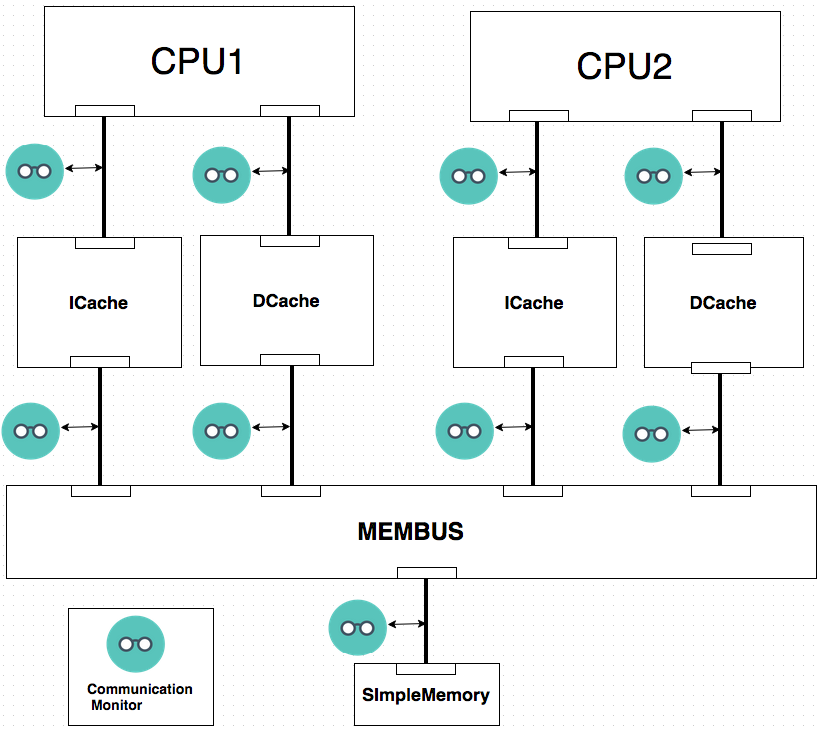
\includegraphics[width=3in]{figures/Fig4.png}}
\caption{SoC platform structure.}
\label{SoC}
\end{figure}

To determine the efficiency of the trace analysis method for
a realistic example, a transaction level model of a SoC is
constructed within the GEM5 environment~\cite{Binkert2011}.
The GEM5 simulator is a modular platform for computer-system architecture research, 
encompassing system-level architecture as well as processor micro-architecture.
This SoC model, as shown in Fig.~\ref{SoC}, consists of two
ARM Cortex-A9 cores, each of which contains two separate
16KB data and instruction caches.  The caches are connected
to a 1GB memory through a memory bus model.  Components
communicate with each other by sending and receiving various
request and response messages.  In order to observe and
trace communications occurring inside this model during
execution, monitors are attached to links connecting the
components.  These monitors record the messages flowing
through the links they are attached to, and store them into
output trace files.

By combining the informations from all of the nine communication monitors, required communication traces are obtained. As a virtualized SoC platform, GEM5 has three types of request: timing, atomic and functional. Timing request include the modeling of queuing delay and resource contention. Atomic request is a faster than timing request with no delay.  Functional request is used for loading binaries, examining/changing variables in the simulated system, and so on. In our case, we specify all our request to be timed as it's the most detailed one.However, some of the system initiation is still atomic and it's not related to our research, so we only took the messages that are timing request from our collected data. 


For this model, we consider the flow specifications
describing the cache coherence protocols supported in
GEM5 that is used to build the model in Fig~\ref{SoC}.
The GEM5 cache coherence protocols can be found at~\cite{gem5}.
These flow specifications describe data/instruction read
operations and data write operations initiated from CPUs.
Three such flows describe the cache coherent protocols for
each CPU.  Since there are two CPUs, there are six flows in
the model.



We wrote two simple concurrent programs, one for each CPU,
 to exercise the flows.  They read numbers from a file,
perform some operations on these numbers, and store the
results back to the file.  How GEM5 supports shared memory
multi-threaded program execution is unclear.  Therefore,
no data are shared in both caches in this test.
Furthermore, GEM5 does not support true concurrency.  When
there are two programs running on the CPUs, GEM5 alternates
the executions between the two CPUs.  To simulate
asynchronous concurrency with the interleaving semantics,
those two simple programs are instrumented with
pseudo-blocking commands, one placed before each statement.
A pseudo blocking command includes a random number generator
that returns either $0$ or $1$ and a loop that only exits
when the returned random number is $0$.

We produce a result file including all of the communication messages between every components from two simple programs running simultaneously on each CPU.  The program assigned to CPU1 read one file three times for one letter and writing one letter for three times to the same file. CPU2's program will do the same read and write functionalities to the same file, only difference is that CPU2 will write first and then read. One thing we should know about GEM5 is that even when we run these two programs concurrently, it will attempt to produce a concurrent result. The data we collected shows that it's not the real nondeterministic concurrency. What GEM5 did was it allowed two CPUs to execute its own instruction in turn, therefore the order was deterministic. Therefore, no matter how many times we ran the program, it produced the same result. We tried other virtual SoC platform softwares, and this was the best nondeterministic concurrency we can get. Even if this is slightly off with what the real chip should work, it still surve our purpose of testing the correctness of our algorithm.


\begin{table}[tb]
\caption{Runtime Results of Trace analysis. Time is in seconds and memory usage is in MB.}
\begin{center}
\begin{tabular}{|c|c|c|c|c|}
\hline
	&	F-Obs. & \begin{tabular}{c}P-Obs. \\ No Amb.\end{tabular} & \begin{tabular}{c}P-Obs. \\ Amb.~1\end{tabular} & \begin{tabular}{c}P-Obs. \\ Amb.~2\end{tabular} \\
\hline
\hline
Time & $3$ & $2.78$ & $896$ & $<1$\\
\hline
Mem & $12$ & $10$ & $420$ & $9$\\
\hline
	
\end{tabular}
\end{center}
\label{table-results}
\end{table}%

After this model is executed with the simple concurrent programs, 
the trace analysis is applied to traces with different observabilities
collected from this model.  The runtime results are shown in Table~\ref{table-results}.
The first column shows the results from analyzing the trace with the full
observability, while the next three show the result from 
analyzing traces with different partial observability assumptions.

In the first experiment, full observability is assumed.
After the SoC model finishes executing the program, there
are totally $343581$ messages collected in the trace file.
Not all of the messages are relevant to the flow
specification as many are used by GEM5 to initialize its
simulation environment.  After removing those irrelevant
messages, the number of messages in the trace file is to
reduced to $121138$.

The time taken to remove the irrelevant messages from the
trace is negligible.  The total runtime and the peak memory
taken by the trace analysis algorithm on the reduced
trace are 3 seconds and 12MB, respectively.  Only one flow execution
scenario is extracted, and 
Table~\ref{table-case-2} shows the number of flow instances contained in that
scenario for the six 
flows describing cache coherent operations initiated from both CPUs.
\begin{table}[tb]
\caption{The number of flow instances derived by the trace analysis with the full observability.}
\begin{center}
\begin{tabular}{|l|c|}
\hline
Flows & $\#$Instances \\
\hline
\hline
CPU1 Data Read			&  $17582$\\
CPU1 Instruction Read		&  $4002$\\
CPU1 Write				&  $3370$\\
\hline
CPU2 Data Read			&  $17386$\\
CPU2 Instruction Read		&  $3955$\\
CPU2 Write				&  $3308$\\
\hline
\end{tabular}
\end{center}
\label{table-case-2}
\end{table}%

In the second experiment, partial observability is taken into account
with the four monitors attached to the links between two CPUs and their
caches are disabled. Then, the trace is generated by the
remaining five monitors from the SoC model executing the
same program.  The new trace contains 15089 messages.  
Similarly, only one flow execution
scenario is extracted, and the numbers of the
flow instances contained in that execution scenario are
shown in Table~\ref{table-par-obs}.  From these results, the
numbers of the flow instances are dropped significantly
compared to the results extracted from the trace with the
full observability as shown in
Table~\ref{table-case-2}. This difference is due to that
some communications occurred in the system when executing
the program involve the CPUs and their corresponding caches
only, and the traffic on the links between the CPUs and
their corresponding caches is not observable. Therefore, the
instances of the flow specifications characterizing these
communications do not exist in the trace. In other words,
all extracted flow instances in Table~\ref{table-par-obs}
characterize the communications that pass through the memory
bus in the system model.  The runtime and memory usage as shown in
the third column in Table~\ref{table-results} are
similar to those for analyzing the trace of the full
observability.

\begin{table}[tb]
\caption{The number of flow instances derived by the trace analysis with certain monitors disabled.}
\begin{center}
\begin{tabular}{|l|c|}
\hline
Flows & $\#$Instances \\
\hline
\hline
CPU1 Data Read			&  $829$\\
CPU1 Instruction Read		&  $169$\\
CPU1 Write				&  $82$\\
\hline
CPU2 Data Read			&  $803$\\
CPU2 Instruction Read		&  $190$\\
CPU2 Write				&  $83$\\
\hline
\end{tabular}
\end{center}
\label{table-par-obs}
\end{table}%

In the third experiment, further partial observability is taken into consideration.  In this experiment, only the five links involving the memory bus are still considered.  However, an assumption is made that all events passing the same link are not distinguishable due to the limited observability.  The monitors are modified such that whenever an event is captured on one of the links, it dumps a set of events passing through the same link into the trace file.  Therefore, each line of the trace file corresponds to a set of events.  After applying the trace analysis to this trace,  a total of 13944 flow execution scenarios are extracted.    This large number, compared to the results from the first two experiments, is due to the ambiguous interpretation of the events with limited observability.  

The whole experiment takes about $15$ minutes and $420$~MB to finish as shown in column~4
in Table~\ref{table-results}, significantly higher than the numbers for analyzing traces where there is no ambiguity in the observed events.  This is due to the fact that a trace of ambiguous events is in fact a set of traces of original events, which lead to large numbers of execution scenarios either during or at the end of the analysis.  In this experiment, the peak number of execution scenarios during the analysis process is $70384$, many of which are invalid and removed eventually.  However, controlling the number of intermediate execution scenarios during the trace analysis is critical in order for the analysis to be tractable.  Here, insights from validators could help, but are not used in this experiment.   

As shown above, the ambiguous interpretation of events can lead to large numbers of intermediate and final execution scenarios, which not only make the trace analysis more time consuming but also make it difficult to gain insightful understanding from the derived execution scenarios.  Careful selection of what to observe may have big impact on results from the trace analysis.  In this last experiment, we relax the assumption made in the previous experiment such that the events passing each link are partitioned into two groups, one for read operations and one for write operations.  Similar to the assumption made in the previous experiment, events in the same group are assumed to be non-distinguishable.  The monitors are modified accordingly such that they output all events in the same group into the trace file if an event from that group is captured.  After the trace analysis on this new partially observed trace is finished, only one execution scenario is derived where the distribution of the numbers of flow instances is the same as those shown in Table~\ref{table-par-obs}.  The peak number of execution scenarios encountered during the trace analysis is $4$.  The total runtime and memory usage are negligible as shown in the last column in Table~\ref{table-results}.  Compared to the results from the previous experiment, the precision and the performance of the trace analysis are improved dramatically as a result of careful selection of observable events. 


\begin{figure} 
\centerline{
\includegraphics[width=7in]{struc.pdf}}
\caption{SoC platform structure.}
\label{rtlstruc}
\end{figure}


\section{Simulation Simple RTL SoC with VHDL}
A register transfer level SoC model is constructed. This model is more specific compared to the last model as the register value will be updated every cycle, thus will be much slower than the model on GEM5. Because the lack of similar research, we couldn't find any existing model, so this model is built from scratch just by me. The desired protocols are implemented inside all the components. Because this is a simplified model, the CPU can't run software programs. A test generator is implemented inside CPU to allow simple functions.

 As showed in Fig.~\ref{rtlstruc}, this model consists of two CPU models, each with its own 1KB cache. The caches are connected to a 4MG memory through a memory bus model. At each rising clock cycle, our model will record selected signal value into a vcd(value change dump) format file.

This model has 6 protocols implemented. It's based on the protocols provided by GEM5 with some modification. 3 types of protocols: read, write and write back is implemented for both CPU. Write back protocol is new and will be invoked when Cache need to flush back dirty datas.

For every clock cycle, the test generator inside each CPU will randomly generate a read or write operation. In order to better active and cache coherent protocol, only first 3 bits of the 16 bits request address are random generated, while the rest of the bits are predefined. By limiting the address to a certain range, it's more likely that one CPU will request data that exists in the other CPU.

In this experiment model, full observability is assumed.
After the SoC model finishes 2000 flows for each cpu, there
are totally $122704$ messages collected in the trace file.
The system takes 10 second to run and the peak memory used is 18MB.

Table~\ref{table-case-3} shows the number of flow instances contained in that
scenario for the six 
flows describing cache coherent operations initiated from both CPUs.
\begin{table}[tb]
\caption{The number of flow instances derived by the trace analysis with the full observability.}
\begin{center}
\begin{tabular}{|l|c|}
\hline
Flows & $\#$Instances \\
\hline
\hline
CPU1 Read			&  $5090$\\
CPU1 Write				&  $4910$\\
CPU1 Write Back				&  $1270$\\

\hline
CPU2 Read			&  $4932$\\
CPU2 Write				&  $5068$\\
CPU2 Write Back				&  $1211$\\
\hline
\end{tabular}
\end{center}
\label{table-case-3}
\end{table}%

During the building of the system, we used our analysis algorithm
as a debugging method to find the problems. Following types of errors
are detected by the algorithm and fixed.
\begin{itemize}
\item 
Error one: interconnect bus sending same request to Memory more than one time. 
During the trace analysis, our algorithm shows that the trace will always stop when interconnect send
 request to Memory and the message cannot be mapped to any existing scenarios. The error message
 looks exactly the same as the previous message. We traced the bug to interconnect and find out the request
 wasn't reset correctly.
 \item
Error two: command changed after interconnect bus receive snoop request from Cache. 
Our trace analysis algorithm find message from cache to memory can't map to any existing scenarios in 
multiple runs, and all the stacked messages are snoop response. By debugging the cache component,
we discovered the wrong implemented cache coherent protocol and fixed the error.
\item
Error three: when running Peterson's Algorithm to ensure mutual exclusion between two processors, our analysis algorithm 
shows no cache coherence protocol was activated. Based on programers experience, there has to be at least one cache 
coherence flow exist because of the shared locks and variable between two CPUs. 
The unmatched number of cache coherence flows shows an big error in our system implementation
of cache coherence protocol.
 
\end{itemize}
\chapter{Conclusion and Future Works}
This thesis presents a method for post-silicon validation by
interpreting observed raw signal traces at the level of
system flow specifications.  The derived flow execution
scenarios provide more structured information on system
operations, which is more understandable to system
validators.  This information can help to locate design
defects more easily, and also provides a measurement of
validation coverage.

Due to partial observability, this approach may derive a
large number of different flow execution scenarios for a
given signal trace.  Insights from system validators can
help to eliminate some false scenarios due to the partial
observability.  An interesting future direction is
formalization of the validators' insights using temporal
logic on flows so that the validators can express their
intents more precisely and concisely.

The trace analysis approach presented in this thesis needs to
be iterated with different observations selected in
different iterations in order to eliminate the false
scenarios and to root cause system failures as quickly as
possible.  The observation selection and stitching signal
traces of different observations together for the above goal
will also be pursued in the future.





\begin{appendix}

\chapter{Flow specifications and protocols provided by GEM5}
\section{Protocol Specifications in Message Sequence Chart}
\begin{figure}[h]
\centering
 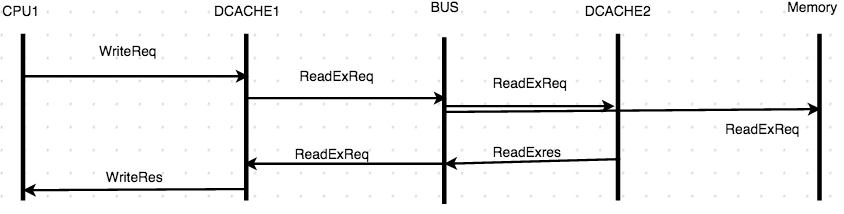
\includegraphics[width=4.5In]{figures/write3.png}
 \caption{\footnotesize Flow sequence chart of write operation when requested data is not included in Dcache. ReadExRes can also be sent from Memory if Dcache2 does not have requested data. This sequence chart is symmetric for CPU2. }
 \label{write3}

 \centering
 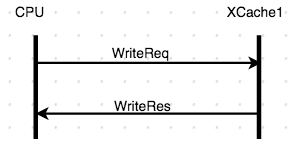
\includegraphics[width=2In]{figures/write1.png}
 \caption{\footnotesize Flow sequence chart of write operation when XCache has the exclusive right of requested data. XCache can be instruction cache or data cache. This sequence chart is symmetric for CPU2. }
 \label{write1}
   \centering
 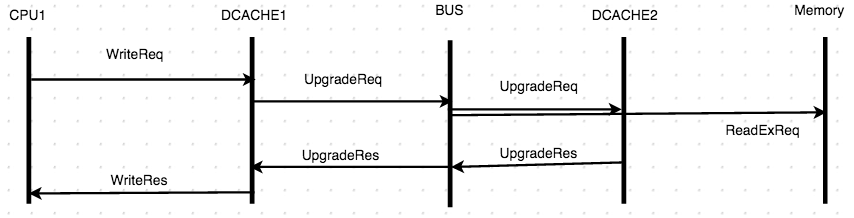
\includegraphics[width=4.6In]{figures/write2.png}
 \caption{\footnotesize Flow sequence chart of write operation when requested data is shared by another component. UpgradeRes can also be sent from Memory if Dcache2 does not have requested data. This sequence chart is symmetric for CPU2. }
 \label{write2}
 \end{figure}
\begin{figure}[h] 
 \centering
 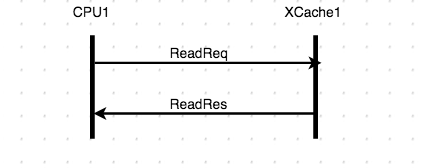
\includegraphics[width=2In]{figures/read1.png}
 \caption{\footnotesize Flow sequence chart of read operation when XCache has the exclusive right of requested data. XCache can be instruction cache or data cache. This sequence chart is symmetric for CPU2. }
 \label{read1}
 
 \centerline{
 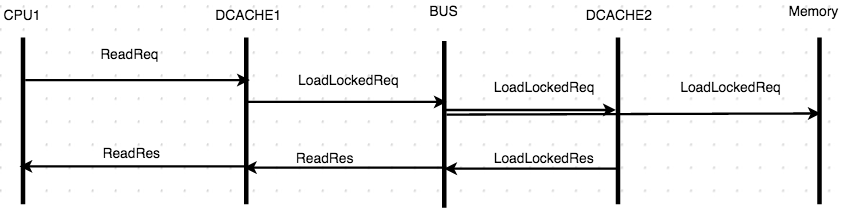
\includegraphics[width=4.1In]{figures/read3.png}}
 \caption{\footnotesize Flow sequence chart of read operation when requested data is shared by another component. LoadLockedRes can also be sent from Memory if Dcache2 does not have requested data. This sequence chart is symmetric for CPU2. }
 \label{read3}

 \centerline{
 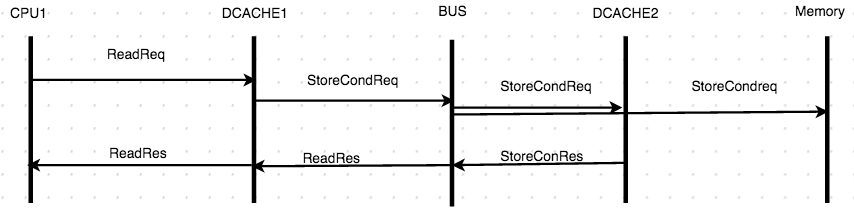
\includegraphics[width=3.9In]{figures/read2.png}}
 \caption{\footnotesize Flow sequence chart of read operation when requested data is not present. StoreCondRes can also be sent from Memory if Dcache2 does not have requested data. This sequence chart is symmetric for CPU2. }
 \label{read2}
 \end{figure}
\newpage
\section{Protocol Specification in LPNs}%
\begin{figure}[h]
\centerline{
 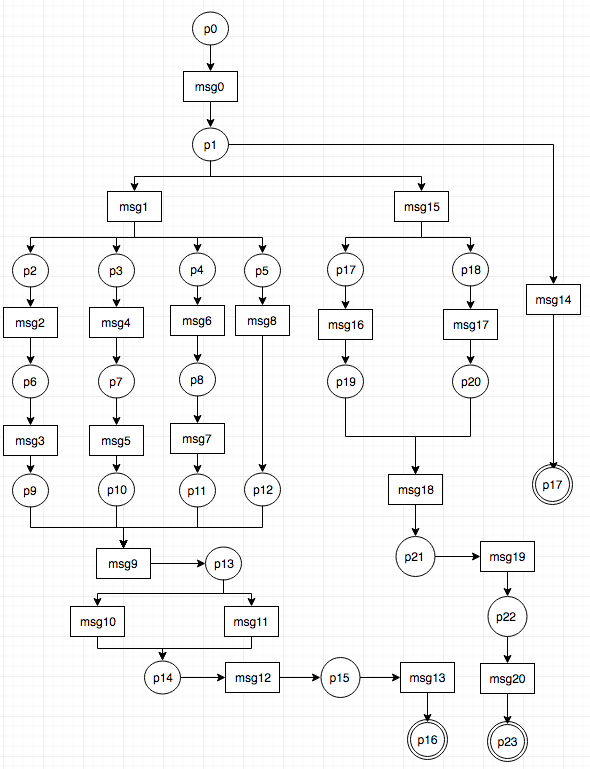
\includegraphics[width=3.1In]{figures/Fig5.png}}%
\begin{minipage}{.5\textwidth}
 {\footnotesize
 \[
 \begin{array}{llll}
 msg_0: (&\mbox{ CPU1},&\mbox{writeReq},&\mbox{icache1   })\\       
 msg_1: (&\mbox{ dcache1},&\mbox{ readExreq },&\mbox{Bus     })\\        
 msg_2: (&\mbox{ Bus},&\mbox{ readExreq},&\mbox{ dcahce2 })\\  
 msg_3: (&\mbox{ dcache2},&\mbox{readExreq},&\mbox{cpu2         })\\   
 msg_4: (&\mbox{ Bus},&\mbox{ readExreq},&\mbox{ icahce2           })\\  
 msg_5: (&\mbox{ icache2},&\mbox{readExreq},&\mbox{cpu2 })\\  
 msg_6: (&\mbox{ Bus},&\mbox{ readExreq},&\mbox{ icahce1       })\\     
 msg_7: (&\mbox{ dcache1},&\mbox{readExreq},&\mbox{cpu1           })\\  
 msg_8: (&\mbox{ Bus},&\mbox{ readExreq},&\mbox{ Memory })\\  
 msg_9: (&\mbox{ true                                          })\\  
 msg_{10}: (&\mbox{ Memory},&\mbox{ readExres},&\mbox{ Bus})
  \end{array}
 \]}
\end{minipage}
\begin{minipage}{.5\textwidth}
 {\footnotesize
 \[
 \begin{array}{llll}
 msg_{11}: (&\mbox{ icache2},&\mbox{ readExres},&\mbox{ Bus })\\  
 msg_{12}: (&\mbox{ Bus},&\mbox{ readExres},&\mbox{ dcache1})\\  
 msg_{13}: (&\mbox{ icache1},&\mbox{ writeRes},&\mbox{ CPU1         })\\  
 msg_{14}: (&\mbox{ icache1},&\mbox{ writeRes},&\mbox{ CPU1 })\\  
 msg_{15}: (&\mbox{ dcache1},&\mbox{UpgradeReq},&\mbox{Bus})\\  
 msg_{16}: (&\mbox{ Bus},&\mbox{ UpgradeReq},&\mbox{ icahce2      })\\   
 msg_{17}: (&\mbox{ Bus},&\mbox{ UpgradeReq},&\mbox{ Memory })\\  
 msg_{18}: (&\mbox{ icache2},&\mbox{UpgradeRes},&\mbox{ Bus     })\\  
 msg_{19}: (&\mbox{ Bus},&\mbox{ UpgradeRes},&\mbox{ dcache1      })\\  
 msg_{20}: (&\mbox{ icache1},&\mbox{ writeRes},&\mbox{ CPU1 })\\
 \\
 \end{array}
 \]}
\end{minipage}
 \caption{\footnotesize Flow specification of a cache coherent write operation initiated from CPU1 to instruction cache. \footnotesize This flow is symmetric for CPU2. }
 \label{write-flow}
 \end{figure}
 \begin{figure}
 \centering
  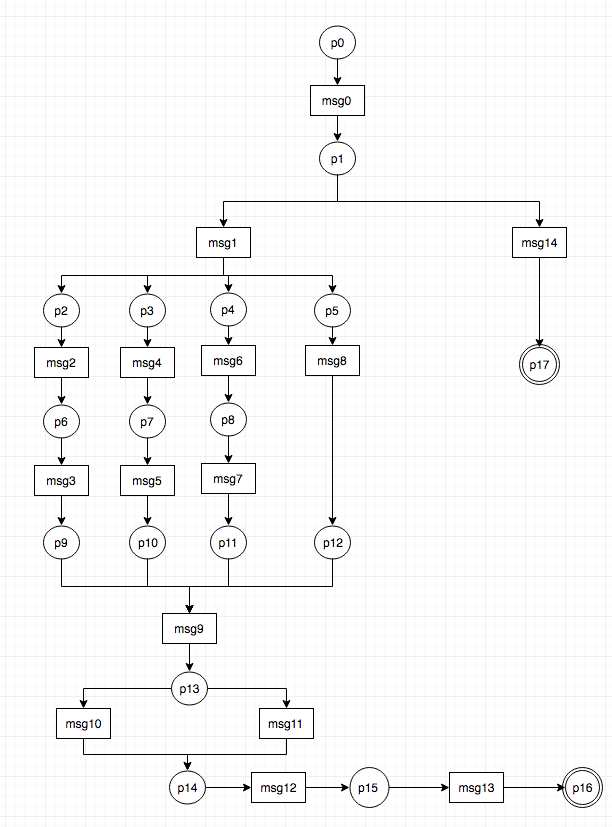
\includegraphics[width=3.3in]{figures/Fih6.png}
  \begin{minipage}{.5\textwidth}
 {\footnotesize
 \[
 \begin{array}{llll}
 msg0: (&\mbox{ CPU1},&\mbox{ReadReq},&\mbox{icache1  })\\                   
 msg1: (&\mbox{ dcache1},&\mbox{ StoreCondreq },&\mbox{Bus })\\           
 msg2: (&\mbox{ Bus},&\mbox{ StoreCondreq},&\mbox{ icahce2 })\\
 msg3: (&\mbox{ icache2},&\mbox{StoreCondreq},&\mbox{cpu2       })\\      
 msg4: (&\mbox{ Bus},&\mbox{ StoreCondreq},&\mbox{ dcahce2           })\\ 
 msg5: (&\mbox{ dcache2},&\mbox{StoreCondreq},&\mbox{cpu2 })\\
 msg6: (&\mbox{ Bus},&\mbox{ StoreCondreq},&\mbox{ dcahce1     })\\       
 msg7: (&\mbox{ icache1},&\mbox{StoreCondreq},&\mbox{cpu1           })
  \end{array}
 \]}
 \end{minipage}%
 \begin{minipage}{.5\textwidth}
  {\footnotesize
 \[
 \begin{array}{llll}
 msg8: (&\mbox{ Bus},&\mbox{ StoreCondreq},&\mbox{ Memory })\\
 msg9: (&\mbox{ true                                        })\\
 msg10: (&\mbox{ Memory},&\mbox{ ReadRes},&\mbox{ Bus            })\\    
 msg11: (&\mbox{ icache2},&\mbox{ ReadRes},&\mbox{ Bus })\\
 msg12: (&\mbox{ Bus},&\mbox{ ReadRes},&\mbox{ dcache1      })\\            
 msg13: (&\mbox{ icache1},&\mbox{ ReadRes},&\mbox{ CPU1          })\\  
 msg14: (&\mbox{ icache1},&\mbox{ ReadRes},&\mbox{ CPU1 })\\\\
 \end{array}
 \]}
 \end{minipage}
 \caption{\footnotesize Flow specification of a cache coherent read operation initiated from CPU1 to instruction cache. \footnotesize This flow is symmetric for CPU2. }
 \label{read-flow} 
 \end{figure}
 
 \begin{figure}[h] 
 \centerline{
 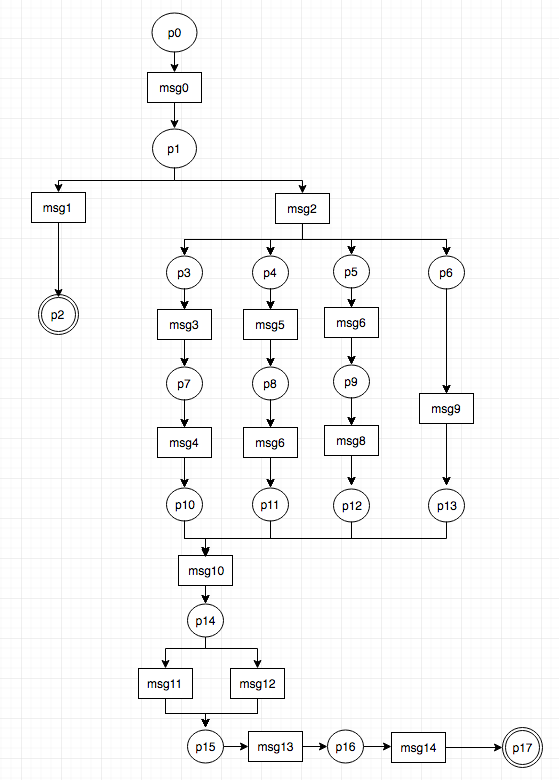
\includegraphics[width=3.3in]{figures/readDcache.png}}
 \begin{minipage}{.5\textwidth}
 {\footnotesize
 \[
 \begin{array}{llll}
 msg0: (&\mbox{ CPU1},&\mbox{ReadReq},&\mbox{dcache1  })\\                   
 msg1: (&\mbox{ dcache1},&\mbox{ ReadRes},&\mbox{ CPU1 })\\
 msg2: (&\mbox{ icache1},&\mbox{ LoadLockedreq },&\mbox{Bus })\\     
 msg3: (&\mbox{ Bus},&\mbox{ LoadLockedreq},&\mbox{ dcahce2     })\\
 msg4: (&\mbox{ dcache2},&\mbox{LoadLockedreq},&\mbox{cpu2 })\\
 msg5: (&\mbox{ Bus},&\mbox{ LoadLockedreq},&\mbox{ icahce2     })\\ 
 msg6: (&\mbox{ icache2},&\mbox{LoadLockedreq},&\mbox{cpu2     })\\
 msg7: (&\mbox{ Bus},&\mbox{ LoadLockedreq},&\mbox{ dcahce1 })

 \end{array}
 \]}
 \end{minipage}\hfill%
  \hfill\begin{minipage}{.5\textwidth}
 
 {\footnotesize
 \[
 \begin{array}{llll}
 msg8: (&\mbox{ icache1},&\mbox{LoadLockedreq},&\mbox{cpu1       })\\
 msg9: (&\mbox{ Bus},&\mbox{ LoadLockedreq},&\mbox{ Memory     })\\
 msg10: (&\mbox{ true })\\
 msg11: (&\mbox{ Memory},&\mbox{ ReadRes},&\mbox{ Bus       })\\     
 msg12: (&\mbox{ icache2},&\mbox{ ReadRes},&\mbox{ Bus    })\\
 msg13: (&\mbox{ Bus},&\mbox{ ReadRes},&\mbox{ icache1 })\\
 msg14: (&\mbox{ dcache1},&\mbox{ ReadRes},&\mbox{ CPU1 })\\\\
 \end{array}
 \]}
 \end{minipage}
 
 \caption{\footnotesize Flow specification of a cache coherent read operation initiated from CPU1 to  data cache. \footnotesize This flow is symmetric for CPU2. }
 \label{read-dcache} 
 \end{figure}
 \clearpage
 




\chapter{Flow Specifications for RTL model}%
\section{Protocol Specification in Message Sequence Charts}
\begin{figure}[h!] 
\centering
 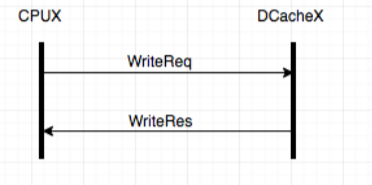
\includegraphics[width=2In]{y1.png}
  \caption{\footnotesize CPU write when cache has exclusive right of the requested data. }
 \label{y1}
 \centering
 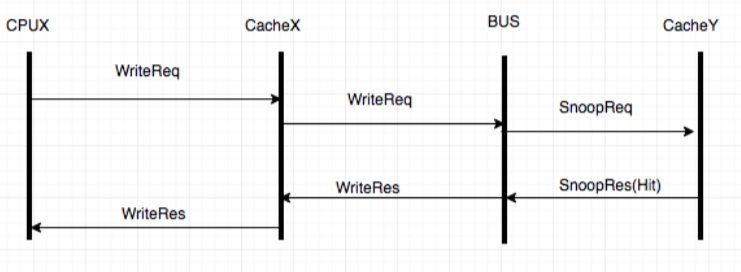
\includegraphics[width=3.6In]{y2.png}
 \caption{\footnotesize CPU write when data only exist in the other CPU's cache }
 \label{y2}
 \centering
 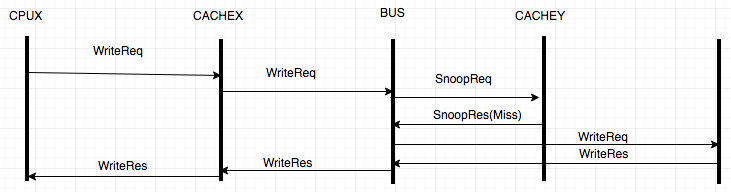
\includegraphics[width=5In]{y3.png}
 \caption{\footnotesize CPU write when requested data only reside in Memory }
 \label{y3}
 \centering
 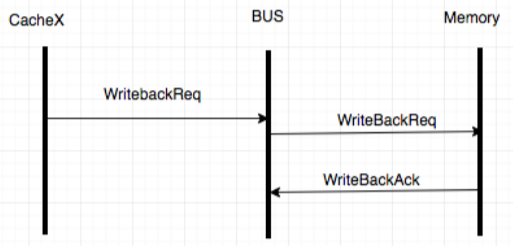
\includegraphics[width=2.8In]{y4.png}
 \caption{\footnotesize Cache send write back request to Memory}
 \label{y4}
\end{figure}

\begin{figure}[h!] 
\centering
 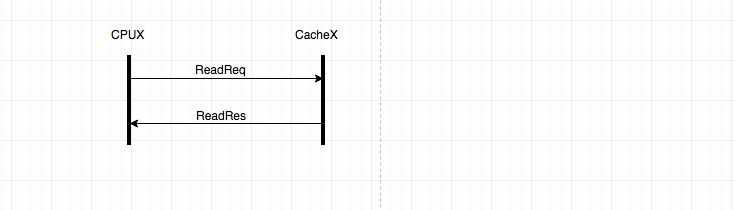
\includegraphics[width=5In]{y5.png}
  \caption{\footnotesize CPU read when cache has exclusive right of the requested data. }
 \label{y4}
 \centering
 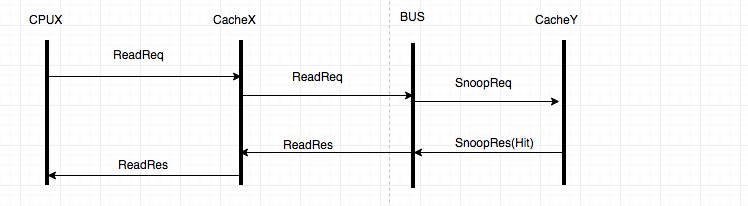
\includegraphics[width=5In]{y6.png}
 \caption{\footnotesize CPU read when data only exist in the other CPU's cache }
 \label{y5}
 \centering
 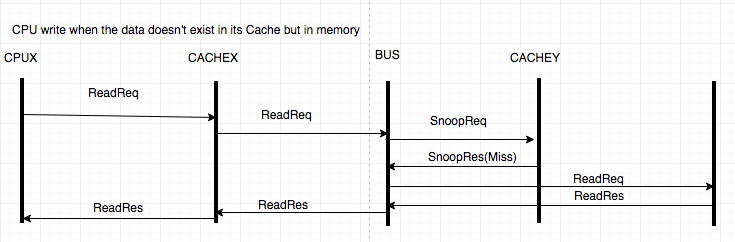
\includegraphics[width=5In]{y7.png}
 \caption{\footnotesize CPU read when requested data only reside in Memory }
 \label{y6}

\end{figure}
 The read and write protocols in RTL model are very similar to what we used in
 GEM5 simulator. However, the command name used here is different.


\section{Protocol Specification in LPNs}

 \begin{figure}[h]
 \centerline{
 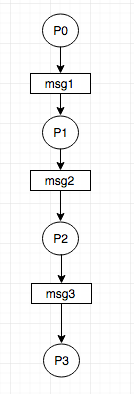
\includegraphics[width=1in]{wbprotocol}}
 {\footnotesize
 \[
 \begin{array}{llll}
 msg1: (&\mbox{ Cache1},&\mbox{ wb },&\mbox{Bus })\\     
 msg2: (&\mbox{ Bus},&\mbox{ wb},&\mbox{ Memory     })\\ 
 msg3: (&\mbox{ Memory},&\mbox{wb},&\mbox{Bus     })\\
 \end{array}
 \]}

  \caption{\footnotesize Flow specification of a cache write back operation initiated from Cache1. \footnotesize This flow is symmetric for CPU2. }
 \label{wbprotocol}
 \end{figure}

\begin{figure}[h]
 \centerline{
 \includegraphics[width=3.2in]{rw}}
 \begin{minipage}{.5\textwidth}
 {\footnotesize
 \[
 \begin{array}{llll}
 msg1: (&\mbox{ CPU1},&\mbox{ wt},&\mbox{ Cache1 })\\
 msg2: (&\mbox{ Cache1},&\mbox{ wt },&\mbox{CPU1 })\\     
 msg3: (&\mbox{ Bus},&\mbox{ snp},&\mbox{ Cache2     })\\
 msg4: (&\mbox{ Cache2},&\mbox{snp},&\mbox{Bus })\\
 msg5: (&\mbox{ Bus},&\mbox{ wt},&\mbox{ Memory     })\\ 
 msg6: (&\mbox{ Memory},&\mbox{wt},&\mbox{Bus     })\\
 \end{array}
 \]}
 \end{minipage}
 \begin{minipage}{.5\textwidth}
 {\footnotesize
 \[
 \begin{array}{llll}
  msg7: (&\mbox{ Bus},&\mbox{ wt},&\mbox{ Cache1 })\\
 msg8: (&\mbox{ Bus},&\mbox{ wt},&\mbox{ Cache1 })\\
 msg9: (&\mbox{ Cache1},&\mbox{wt},&\mbox{CPU1       })\\
 msg10: (&\mbox{ Cache1},&\mbox{wt},&\mbox{CPU1       })\\
 msg11: (&\mbox{ Cache1},&\mbox{wt},&\mbox{CPU1       })\\\\
 \end{array}
 \]}
 \end{minipage}
 \caption{\footnotesize Flow specification of a cache coherent write operation initiated from CPU1 to Cache. \footnotesize This flow is symmetric for CPU2. }
 \label{wtprotocol}
 \end{figure}
\begin{figure}[h]
 \centerline{
 \includegraphics[width=3.2in]{rw}}
\begin{minipage}{.5\textwidth}
 {\footnotesize
 \[
 \begin{array}{llll}
 msg1: (&\mbox{ CPU1},&\mbox{ rd},&\mbox{ Cache1 })\\
 msg2: (&\mbox{ Cache1},&\mbox{ rd },&\mbox{Bus })\\     
 msg3: (&\mbox{ Bus},&\mbox{ snp},&\mbox{ Cache2     })\\
 msg4: (&\mbox{ Cache2},&\mbox{snp},&\mbox{Bus })\\
 msg5: (&\mbox{ Bus},&\mbox{ rd},&\mbox{ Memory     })\\ 
 msg6: (&\mbox{ Memory},&\mbox{rd},&\mbox{Bus     })\\
 \end{array}
 \]}
 \end{minipage}%
 \begin{minipage}{.5\textwidth}
 {\footnotesize
 \[
 \begin{array}{llll}
 msg7: (&\mbox{ Bus},&\mbox{ rd},&\mbox{ Cache1 })\\
 msg8: (&\mbox{ Bus},&\mbox{ rd},&\mbox{ Cache1 })\\
 msg9: (&\mbox{ Cache1},&\mbox{rd},&\mbox{CPU1       })\\
 msg10: (&\mbox{ Cache1},&\mbox{rd},&\mbox{CPU1       })\\
 msg11: (&\mbox{ Cache1},&\mbox{rd},&\mbox{CPU1       })\\\\
 \end{array}
 \]}
 \end{minipage}
 \caption{\footnotesize Flow specification of a cache coherent read operation initiated from CPU1 to Cache. \footnotesize This flow is symmetric for CPU2. }
 \label{readprotocol}
 \end{figure}
 
 
There will be 3 protocols in total: read , write and write back protocl.

All the write operations are implemented in protocol presented in Fig.~\ref{wtprotocol}.
When the request activate cache coherent protocol, like in Fig.~\ref{y2}, it will end in $state 17$. The rest will end in $state 9$ .


All read operations are implemented in protocol presented in Fig.~\ref{readprotocol}. Specification in Fig.~\ref{y6} will end in $state 17$. 
The rest of the specification without activating cache coherence protocol end in $state 9$.

\end{appendix}


\begin{spacing}{1}
\bibliographystyle{unsrt}
\bibliography{SoC}
\end{spacing}

\end{document}
